%%%%%%%%%%%%%%%%%%%%%%%%%%%%%%%%%%%%%%%%%
% Structured General Purpose Assignment
% LaTeX Template
%
% This template has been downloaded from:
% http://www.latextemplates.com
%
% Original author:
% Ted Pavlic (http://www.tedpavlic.com)
%
% Note:
% The \lipsum[#] commands throughout this template generate dummy text
% to fill the template out. These commands should all be removed when 
% writing assignment content.
%
%%%%%%%%%%%%%%%%%%%%%%%%%%%%%%%%%%%%%%%%%

%% mod. by Stefan Seifried

%----------------------------------------------------------------------------------------
%	PACKAGES AND OTHER DOCUMENT CONFIGURATIONS
%----------------------------------------------------------------------------------------

\documentclass{article}

\usepackage{fancyhdr} % Required for custom headers
\usepackage{lastpage} % Required to determine the last page for the footer
\usepackage{extramarks} % Required for headers and footers
\usepackage{graphicx} % Required to insert images
\usepackage{lipsum} % Used for inserting dummy 'Lorem ipsum' text into the template
\usepackage{caption} % figure captions
\usepackage{subcaption} % Required for subfigures
\usepackage{hyperref} %url

% Margins
\topmargin=-0.45in
\evensidemargin=0in
\oddsidemargin=0in
\textwidth=6.5in
\textheight=9.0in
\headsep=0.25in 

\linespread{1.1} % Line spacing

% Set up the header and footer
\pagestyle{fancy}
\lhead{\hmwkAuthorName} % Top left header
\chead{\hmwkClass\ -- \hmwkTitle} % Top center header
\rhead{\firstxmark} % Top right header
\lfoot{\lastxmark} % Bottom left footer
\cfoot{} % Bottom center footer
\rfoot{Page\ \thepage\ of\ \pageref{LastPage}} % Bottom right footer
\renewcommand\headrulewidth{0.4pt} % Size of the header rule
\renewcommand\footrulewidth{0.4pt} % Size of the footer rule

\setlength\parindent{0pt} % Removes all indentation from paragraphs

%----------------------------------------------------------------------------------------
%	DOCUMENT STRUCTURE COMMANDS
%	Skip this unless you know what you're doing
%----------------------------------------------------------------------------------------

% Header and footer for when a page split occurs within a problem environment
\newcommand{\enterProblemHeader}[1]{
\nobreak\extramarks{#1}{#1 continued on next page\ldots}\nobreak
\nobreak\extramarks{#1 (continued)}{#1 continued on next page\ldots}\nobreak
}

% Header and footer for when a page split occurs between problem environments
\newcommand{\exitProblemHeader}[1]{
\nobreak\extramarks{#1 (continued)}{#1 continued on next page\ldots}\nobreak
\nobreak\extramarks{#1}{}\nobreak
}

\setcounter{secnumdepth}{0} % Removes default section numbers
\newcounter{homeworkProblemCounter} % Creates a counter to keep track of the number of problems

\newcommand{\homeworkProblemName}{}
\newenvironment{homeworkProblem}[1][Problem \arabic{homeworkProblemCounter}]{ % Makes a new environment called homeworkProblem which takes 1 argument (custom name) but the default is "Problem #"
\stepcounter{homeworkProblemCounter} % Increase counter for number of problems
\renewcommand{\homeworkProblemName}{#1} % Assign \homeworkProblemName the name of the problem
\section{\homeworkProblemName} % Make a section in the document with the custom problem count
\enterProblemHeader{\homeworkProblemName} % Header and footer within the environment
}{
\exitProblemHeader{\homeworkProblemName} % Header and footer after the environment
}

\newcommand{\problemAnswer}[1]{ % Defines the problem answer command with the content as the only argument
\noindent\framebox[\columnwidth][c]{\begin{minipage}{0.98\columnwidth}#1\end{minipage}} % Makes the box around the problem answer and puts the content inside
}

\newcommand{\homeworkSectionName}{}
\newenvironment{homeworkSection}[1]{ % New environment for sections within homework problems, takes 1 argument - the name of the section
\renewcommand{\homeworkSectionName}{#1} % Assign \homeworkSectionName to the name of the section from the environment argument
\subsection{\homeworkSectionName} % Make a subsection with the custom name of the subsection
\enterProblemHeader{\homeworkProblemName\ [\homeworkSectionName]} % Header and footer within the environment
}{
\enterProblemHeader{\homeworkProblemName} % Header and footer after the environment
}

\newcommand{\code}[1]{\texttt{\textbf{#1}}}
   
%----------------------------------------------------------------------------------------
%	NAME AND CLASS SECTION
%----------------------------------------------------------------------------------------

\newcommand{\hmwkTitle}{Preparatory Task} % Assignment title
\newcommand{\hmwkClass}{Engineering Self-Adaptive Systems} % Course/class
\newcommand{\hmwkAuthorName}{Stefan Seifried} % Your name
\newcommand{\hmwkMatrNr}{00925401} % Your matricle number

%----------------------------------------------------------------------------------------
%	TITLE PAGE
%----------------------------------------------------------------------------------------

\title{
\vspace{2in}
\textmd{\textbf{\hmwkClass:\ \\ \hmwkTitle}}\\
\vspace{3in}
}

\author{
	\textbf{\hmwkAuthorName} \\
	\textbf{Matr.Nr.: \hmwkMatrNr}
}
\date{} % Insert date here if you want it to appear below your name

%----------------------------------------------------------------------------------------

\begin{document}

\maketitle

%----------------------------------------------------------------------------------------
%	TABLE OF CONTENTS
%----------------------------------------------------------------------------------------

%\setcounter{tocdepth}{1} % Uncomment this line if you don't want subsections listed in the ToC

%% SES: table of contents not really needed

%\newpage
%\tableofcontents
\newpage

%----------------------------------------------------------------------------------------
%	UPPAAL - LESSONS LEARNED
%----------------------------------------------------------------------------------------
\section{Uppaal -- Lessons Learned}

Uppaal \footnote{\url{http://www.uppaal.org/}} is an integrated tool environment for modeling, simulation, and verification of systems that can be modeled as networks of timed automata. A timed automaton is a finite-state machine
extended with dense clock variables (i.e., real numbers) progressing synchronously. The state of a system is then defined by the current state of all automata, the values of the clocks, and the values of variables (e.g., integer or boolean variables). Transitions between different states either are independent or simultaneously with another automaton through the means of synchronization channels. A synchronization channel (e.g., \code{x}) is always comprised of a sender and a receiver where the state transition of the sender (e.g., \code{x!}) introduces a state transition at the receiver (e.g., \code{x?}). The use of transitions between different states can also be limited by the use of guard statements (e.g., guard \code{x>0}). These statements serve as invariants (on clock or ordinary variables) and decide whether a transition may be taken or not (i.e., transition is enabled). Further, clocks and variables may be modified upon a transition (assignments). 

The locations in Uppaal, allow for more fine-grained tuning of their temporal behavior. Despite the explicitly flagged \textit{initial} location, there are three different types of locations: \textit{normal}, \textit{urgent}, and \textit{committed}. \textit{Normal locations} may be used with or without invariants. Meaning that unless there is a restriction enforced by an invariant or a trigger by a synchronization channel, the process may stay in this location indefinitely. \textit{Urgent locations} are semantically equivalent to adding an extra clock x, that is reset on all incoming edges, and having an invariant x<=0 on the location. Hence, time is not allowed to pass when the system is in an urgent location. \textit{Committed locations} are even more restrictive on the execution than \textit{urgent locations}. A state is committed if any of the locations in the state is \textit{committed}. A \textit{committed} state cannot delay, and the next transition must involve an outgoing edge of at least one of the \textit{committed locations} (See Section 2.1 in \cite{Tut01}).

%----------------------------------------------------------------------------------------
%	SIMPLE LAMP
%----------------------------------------------------------------------------------------
\section{Simple lamp}

Figure~\ref{fig:SimpleLamp} shows two automata modeling the simple lamp system as described in \cite{Tut01}. The \textit{simple lamp} example consists of two independent processes, the \textit{User}, and the \textit{Lamp}. The User can control the lamp with button presses to change the state of the Lamp to either \textit{off}, \textit{low} or \textit{bright}. The \textit{Lamps} \textit{bright} state can only be reached by two consecutive presses within the duration of 5-time units. The full source code of the implementation can be found at GitHub \footnote{\url{https://github.com/daFritz84/Engineering-Self-Adaptive-Systems}}.

\begin{figure}[h!]
	\centering
	\begin{subfigure}{.5\textwidth}
		\centering
		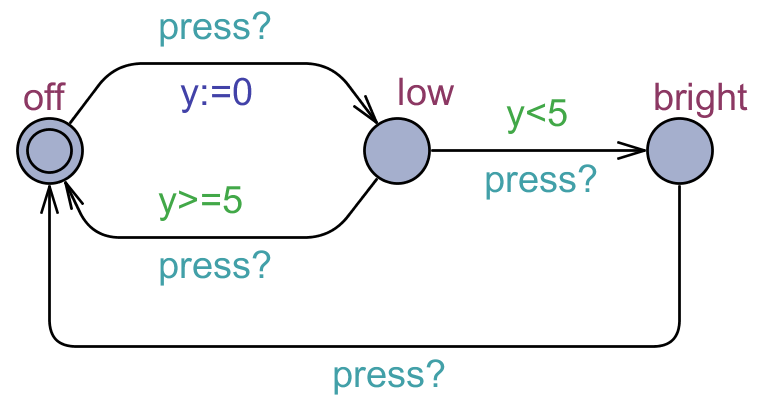
\includegraphics[width=.9\linewidth]{Lamp/figTLamp}
		\caption{Lamp}
	\end{subfigure}
	\begin{subfigure}{.3\textwidth}
		\centering
		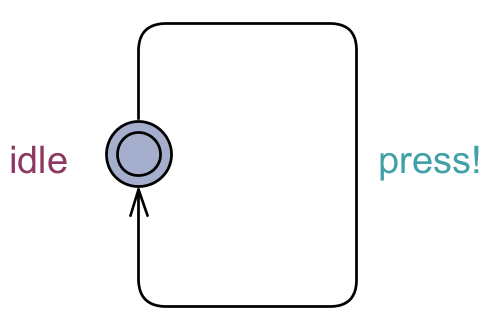
\includegraphics[width=.9\linewidth]{Lamp/figTUser}
		\caption{User}
	\end{subfigure}
	\caption{The simple lamp example}
	\label{fig:SimpleLamp}
\end{figure}

\subsection{Task -- Step 6: Prove deadlock freedom}

Task 6 stated that the deadlock freedom of the simple lamp example should be proven utilizing the default query provided by Uppaal. This query, \code{A[] not deadlock} can be found either in the simple tutorial \cite{Tut02}, the detailed tutorial \cite{Tut01}, or by looking for \textit{deadlock} in the Uppaal help file. In Uppaal, a \code{deadlock} is a special state formula, which is satisfied for all deadlock states. A state is a deadlock state if
there are no outgoing action transitions neither from the state itself or any of
its delay successors (see detailed tutorial, section 2.2 \cite{Tut01}). To prove the deadlock freedom of our automata, the \code{deadlock} state formula must not hold for any reachable state. Therefore, Uppaal offers \code{A[] $\phi$} (\cite{Tut01}) path formula, where the state $\phi$ must hold for all paths. Combining the state and path formula, the resulting query is created \code{A[] not deadlock} which ultimately means: For all paths the \textit{deadlock} property does not hold.

%----------------------------------------------------------------------------------------

%----------------------------------------------------------------------------------------
%	SIMPLE LAMP WITH LAMPCONTROLLER
%----------------------------------------------------------------------------------------
\section{Simple lamp with lamp controller}

Figure \ref{fig:SimpleLampController} depicts the three automata modeling the enhancements to the original simple lamp example. The requirements in Task - Step 7 stated that the control of the lamp should now be handled by an intermediary process, the \textit{lamp controller}. Hence, three new synchronization channels were introduced to trigger transitions to the different locations of the lamp process, namely \textit{off}, \textit{low}, and \textit{bright}. Therefore, the lamp automaton is simplified, since it now lacks the transitions necessary for the double-press mechanism. The lamp controller mostly follows the model from the original simple lamp example. A striking repeated modeling pattern of the lamp controller automata is its use of committed locations. These locations had to be inserted to separate the \textit{press} synchronization channel with the triggered synchronization channel (i.e., \textit{off}, \textit{low}, or \textit{bright}). Again the full source code of the example can be found on GitHub \footnote{\url{https://github.com/daFritz84/Engineering-Self-Adaptive-Systems}}. 

\begin{figure}[h!]
	\centering
	\begin{subfigure}{.5\textwidth}
		\centering
		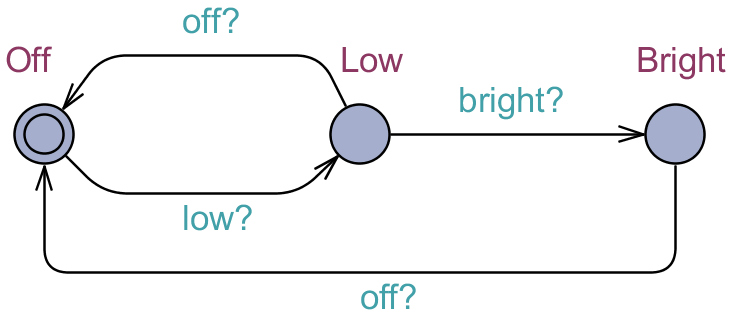
\includegraphics[width=.9\linewidth]{LampController/figTLamp}
		\caption{Lamp}
	\end{subfigure}
	\begin{subfigure}{.3\textwidth}
		\centering
		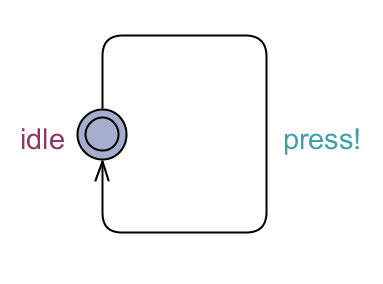
\includegraphics[width=.9\linewidth]{LampController/figTUser}
		\caption{User}
	\end{subfigure}
	\begin{subfigure}{.7\textwidth}
		\centering
		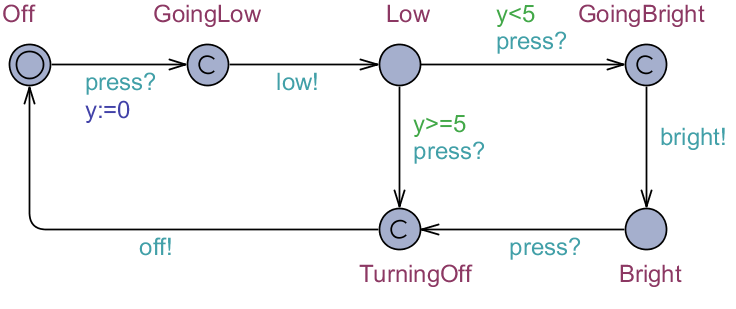
\includegraphics[width=.9\linewidth]{LampController/figTLampController}
		\caption{LampController}
	\end{subfigure}
	\caption{The simple lamp with lamp controller example}
	\label{fig:SimpleLampController}
\end{figure}

Another part of the assignment -- step 7 was the creation of two queries which prove the reachability of the locations low and bright. Reachability in Uppaal is defined as that there exists a path in an automata where the state formula $\phi$ is possibly satisfied \cite{Tut01}. This task is realized by the following two queries:

\begin{description}
	\item[\code{E<> Lamp.Low}] There exists a path where \code{Lamp.Low} eventually holds. Where \code{Lamp.Low} only holds if in fact the corresponding location in the \textit{lamp} automata has been reached.
	\item[\code{E<> Lamp.Bright}] There exists a path where \code{Lamp.Bright} eventually holds.
	Where \code{Lamp.Bright} only holds if in fact the corresponding location in the \textit{lamp} automata has been reached.
\end{description}

%----------------------------------------------------------------------------------------

%----------------------------------------------------------------------------------------
%	REFERENCES
%----------------------------------------------------------------------------------------
\begin{thebibliography}{2}
	\bibitem{Tut01} Gerd Behrmann, Alexandre David, and Kim G. Larsen, \textit{A Tutorial on Uppaal 4.0}, 2006.
	\bibitem{Tut02} \textit{Uppaal 4.0 : Small Tutorial}, 2009
\end{thebibliography}

%----------------------------------------------------------------------------------------

\end{document}
